\subsection{State-space representation of the disturbance}
\label{statespace_disturbance}

Although there are several different ways to describe disturbances in control systems, in the presented report one approach is to assume that the power-flow of the inverter and the load can be described by differential equations. It is worth mentioning again that the behavior of the two different disturbances are significantly different. While the additional power-flow from the inverter can be approximated reasonably by a slowly-varying signal, the change in the load is much faster and in most of the cases is assumed to be completely unknown. Despite of the fact that there might be big changes in the load, in the introduction, and while introducing the principle of disturbances in state space, it is assumed to be constant. 

%\begin{figure}[H]
%\centering
%\includegraphics[width=0.3\textwidth]{rapport/billeder/disturbances}
%\caption{Disturbances acting on the plant}
%\label{fig:disturbances}
%\end{figure}

\begin{figure}[H]
\centering
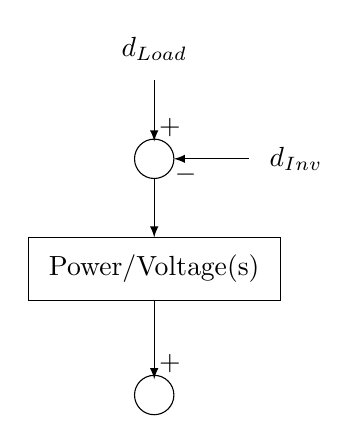
\begin{tikzpicture}

 \draw [-latex] (-0.4,2) ellipse (0.25 and 0.25);
 \draw [-latex] (-2,4) rectangle (1.2,3.2);
 \node at (-0.4,3.6) {\normalsize{Power/Voltage(s)}};
\draw [-latex](-0.4,3.2) -- (-0.4,2.2);
 \node at (-0.2,2.4) {$+$};
 \draw [-latex] (-0.4,5) ellipse (0.25 and 0.25);
\draw [-latex](-0.4,4.75) -- (-0.4,4);
\draw [-latex](-0.4,6) -- (-0.4,5.22);
\node at (-0.4,6.4) {$d_{Load}$};
\draw [-latex](0.8,5) -- (-0.15,5);
\node at (1.4,5) {$d_{Inv}$};
\node at (-0.2,5.4) {$+$};
\node at (0,4.8) {$-$};
\end{tikzpicture}
\caption{Disturbances acting on the plant.}
\label{fig:disturbances}
\end{figure}

As can be seen in \figref{fig:disturbances}, a conversion is required from power to voltage with certain dynamics. However when introducing the disturbances in state space, this dynamic behaviour is neglected and is taken into consideration in the simulation instead. Furthermore, the disturbances acting on the plant will be denoted by $d$ in order to make referencing easier in the further description . 

The disturbance that enters the state-space system can be considered as: 
\begin{equation}
  \label{eq:ss_dist_intro}
    \mathbf{\dot{x}(t)} = \mathbf{A} \mathbf{x}(t) + \mathbf{B} [u(t) + d(t)]
  \end{equation}

In \eqref{eq:ss_dist_intro} $d(t)$ is the disturbance signal which can be characterized by a specific differential equation or transfer function, which can be represented as an individual state-space system. Since the disturbance does not take any inputs, it only provides input for the state-space system of the plant according to \eqref{eq:ss_dist_intro}. The system for the disturbance is called an exo-system and is therefore represented in a form as follows:
%
\begin{equation}
  \label{eq:ss_exo1}
    \mathbf{\dot{x}_d(t)} = \mathbf{A_d} \mathbf{x_d}(t)
  \end{equation}
%
\begin{equation}
  \label{eq:ss_exo2}
    d(t) = \mathbf{C}_d \mathbf{x}_d(t)
  \end{equation}
%
The relation between a state-space model and its transfer function can be described by 
%
\begin{equation}
  \label{eq:ss_tf}
    D(s) = \mathbf{C}_d(s\mathbf{I}-\mathbf{A_d})^{-1} \mathbf{x_d}(0) = \mathbf{C}_d \frac{Adj(s\mathbf{I}-\mathbf{A_d})}{det(s\mathbf{I}-\mathbf{A_d})} \mathbf{x_d}(0) = \frac{f(0,s)}{\Gamma_d(s)}
  \end{equation}
  % 
\begin{minipage}[t]{0.20\textwidth}
Where\\
\hspace*{8mm} $f(0,s)$ \\
\hspace*{8mm} $\Gamma_d(s)$ \\
\hspace*{8mm} and $\mathbf{x_d}(0)$  
\end{minipage}
\begin{minipage}[t]{0.68\textwidth}
\vspace*{2mm}
is the polynomial in s arises because of initial conditions,\\
is called the disturbance generating polynomial, \\
is the vector of initial conditions. 

\end{minipage}

As can be seen, the disturbance generator is the characteristic polynomial of $A_d$. In order to build up the state-space matrices, \eqref{eq:ss_tf} can be split into two equations:
%
\begin{equation}
  \label{eq:ss_tf1}
    \Gamma_d(s) = det(s\mathbf{I}-\mathbf{A_d}) 
  \end{equation}
%
Where $\Gamma_d(s)$ can be considered as the denominator of the transfer function of the disturbance. Therefore $A_d$ can be found easily by solving a simple eigenvalue problem. The equation for the numerator can be written as: 
%
\begin{equation}
  \label{eq:ss_tf2}
    f(0,s) = \mathbf{C}_d Adj(s\mathbf{I}-\mathbf{A_d}) \mathbf{x_d}(0)
  \end{equation}
%
Where $f(0,s)$ represents the numerator of the transfer function of disturbance. $\mathbf{A_d}$ is known from \eqref{eq:ss_tf1} and $\mathbf{x_d}(0)$ consists of the priorly defined initial conditions. Therefore $\mathbf{C}_d$ can be calculated which means that the state representation of the disturbance becomes fully defined. It should be noted however, that even from \eqref{eq:ss_tf} or \eqref{eq:ss_tf2} it can be clearly seen, that if there is not any initial conditions defined for the disturbance, the elements of $\mathbf{C}_d$ are going to be zero. This directly means that there will not be any output of the exo-system, therefore there will not be any disturbance appearing on the output signal. 

According to \eqref{eq:ss_dist_intro}, \eqref{eq:ss_exo1} and \eqref{eq:ss_exo2}, the system can be rewritten in matrix form with the modified matrices including the exo-system: 
%
\begin{equation}
\label{eq:ss_dist1}
\begin{bmatrix}
    \mathbf{\dot{x}} \\
    \mathbf{\dot{x_d}} 
\end{bmatrix}
=
\underbrace{
 \begin{bmatrix}
    \mathbf{A} & \mathbf{B}\mathbf{C_d} \\
    0 & \mathbf{A_d}
\end{bmatrix}
}_\text{\normalsize{$\tilde{\mathbf{A}}$}}
\underbrace{
 \begin{bmatrix}
    \mathbf{x} \\
    \mathbf{x_d}
\end{bmatrix}
}_\text{\normalsize{$\tilde{x}$}}
+
\underbrace{
 \begin{bmatrix}
    \mathbf{B}  \\
    0 &  
\end{bmatrix}
}_\text{\normalsize{$\tilde{\mathbf{B}}$}}
    u
\end{equation}

\begin{equation}
\label{eq:ss_dist2}
    d
=
\underbrace{
 \begin{bmatrix}
    \mathbf{C} & 0 
\end{bmatrix}
}_\text{\normalsize{$\tilde{\mathbf{C}}$}}
 \begin{bmatrix}
    \mathbf{x} \\
    \mathbf{x_d}
\end{bmatrix}
\end{equation}

Therefore an extended state-space model is given where both the states of the plant and the disturbance are taken into account. It should be noted however, that the augmented system is not controllable from the input $d$ because the disturbance by the exo-system is an exogenous, autonomous input. The modified system can be illustrated such as in \figref{fig:exosystem}: 

%\begin{figure}[H]
%\centering
%\includegraphics[width=0.7\textwidth]{rapport/billeder/exosystem}
%\caption{Exo-system as the input of the system}
%\label{fig:exosystem}
%\end{figure}


\begin{figure}[H]
\centering
\begin{tikzpicture}


 \draw [-latex] (-0.4,2) ellipse (0.25 and 0.25);
\node at (1.2,0.2) {\normalsize{$A$}};
\node at (-1.8,2) {\normalsize{$B$}};
\node at (3.2,2) {\normalsize{$C$}};
\node at (-1.8,3.4) {\normalsize{$B$}};
\node at (-5.4,2) {\normalsize{$A_d$}};
\node at (-3.6,3.4) {\normalsize{$C_d$}};
\node at (1.2,2) {\normalsize{$\int$}};

\draw [-latex] (0.8,2.4) rectangle (1.6,1.6);
\draw [-latex] (0.8,0.6) rectangle (1.6,-0.2);
\draw [-latex] (2.8,2.4) rectangle (3.6,1.6);
\draw [-latex] (-2.2,2.4) rectangle (-1.4,1.6);
\draw [-latex] (-2.2,3.8) rectangle (-1.4,3);
\draw [-latex](-1.4,2) -- (-0.6,2);
\draw [-latex](-0.15,2) -- (0.8,2);


\draw [-latex](1.6,2) -- (2.8,2);
\draw [-latex](3.6,2) -- (4.6,2);
\draw [-latex](2.2,2) -- (2.2,0.2) -- (1.6,0.2);
\draw [-latex](0.8,0.2) -- (-0.4,0.2) -- (-0.4,1.8);
\draw [-latex](-1.4,3.4) -- (-0.4,3.4) -- (-0.4,2.2);

\node at (-5.4,3.4) {\normalsize{$\int$}};

\draw [-latex] (-4,3.8) rectangle (-3.2,3);
\draw [-latex] (-5.8,3.8) rectangle (-5,3);
\draw [-latex] (-5.8,2.4) rectangle (-5,1.6);
\draw [-latex](-3.2,3.4) -- (-2.2,3.4);
\draw [-latex](-3.2,2) -- (-2.2,2);
\draw [-latex](-5,3.4) -- (-4,3.4);
\draw [-latex](-4.4,3.4) -- (-4.4,2) -- (-5,2);
\draw [-latex](-5.8,2) -- (-6.4,2) -- (-6.4,3.4) -- (-5.8,3.4);
\node at (-2.8,3.6) {\normalsize{$d$}};
\node at (-2.8,2.2) {\normalsize{$u$}};
\node at (4,2.2) {\normalsize{$y$}};
\draw [dash pattern=on 2pt off 3pt on 4pt off 4pt] (-7.6,4.4) rectangle (-3.2,1);
\node at (-4.2,1.2) {\normalsize{$Exosystem$}};
\end{tikzpicture}

\caption{Exo-system as the input of the system.}
\label{fig:exosystem}
\end{figure}




